\chapter{Domain Separation Networks} \label{ch:dsn}
Increasingly, there are scenarios where we, purposely or inevitably, use data from different domains to train and use a system. Using domain adaptation can help improving the performance of the system as already proven by several previous attempts with various methods \cite{DAGanin, DASurvey}. The Domain Separation Network \cite{DSN} is a neural network that applies domain adaptation effectively and even surpassed some of the previous methods. 

There are many strategies of domain adaptation, e.g. by learning domain-invariant features or by mapping source to target domain. The DSN, like some other architectures, learns so that the representations of the images from source and target domain are similar to each other - the classifier can classify objects independently from its domain. The crucial addition to DSN is that it learns both the components shared by source and target domains and the components only related to a single domain. This way, the network would not mix up the noise coming from shared components of the domains to the representation related to the actual objects that are also common to all domains. 

To better understand DSN, we first need to understand its building blocks and foundations. In this chapter, its own structure, the loss functions involved in its training and the components used in this architecture, which are crucial to the experiments, such as Domain Adversarial Neural Networks (DANN) \cite{dannGanin}, will be discussed in detail. The first section begins with the main structure of the Domain Separation Networks.
 
\section{Structure of Domain Separation Networks} \label{sec:dsnStruct}

\begin{figure}[tbh]
  \centering
    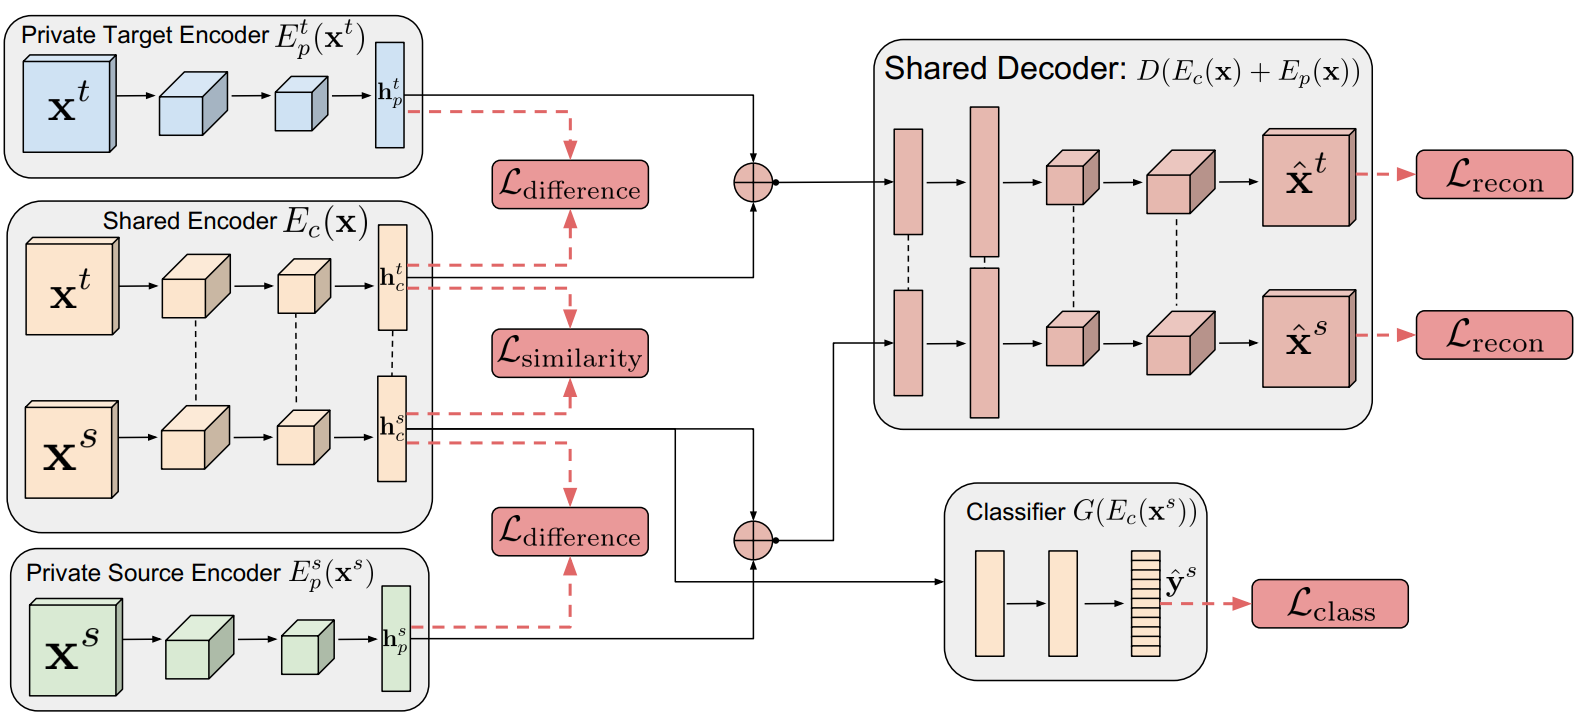
\includegraphics[width=\textwidth]{abbildungen/DSN.png}
  \caption{Main Structure of Domain Separation Networks: A DSN contains private encoders for both domains, ${E_p}^t(x^t)$ for the target domain and ${E_p}^s(x^s)$ for the source domain, a shared encoder $E_c(x)$ creating representations shared across the domains, shared decoder that reconstructs both private representations and evaluate the loss and finally, the classifier $G\left(E_c(x^s)\right)$ that classifies the images based on supervised input images from the source domain.}
  \label{fig:DSN}
\end{figure}

Figure \ref{fig:DSN} shows the structure of the DSN. The network is built up with its private encoders responsible to the source and the target domain, the shared encoder handling the shared representation, the shared decoder that validates the private representations by calculating reconstruction losses, and the classifier trained on the labeled images from the source domain. 

A DSN supports domain adaptation by separately creating representations of the images specific to just the source or target domain, as well as representations shared by both domains. These representations are extracted by the encoders whose functions are described in Section \ref{sec:autoencoders}. Then, since the private representations should be different from each other as possible and should contain generally the characteristics of each domain, the authors add reconstruction losses to ensure that the private representations and the shared representations created by the private encoders are still relevant to the domain it represents. The goal of this separation is to enable the classifier to train on the shared representation, which should be classifiable independently from the domains, without contamination from the representations unique to any of the domains. 

To train the network, the authors use an overall loss function containing four different losses: task loss, reconstruction loss, difference loss, and similarity loss. Since the DANN is used to induce the similarity loss, its structure and function must be explained first before these loss functions are explained in detail in Section \ref{sec:dsnLoss}.

%DANN
\subsection{Domain Adversarial Neural Networks} \label{sec:dann}
The domain adversarial neural network (DANN) \cite{dannGanin} is inspired directly from the idea of domain adaptation suggesting that the prediction made on representation with unclear domain of origin - neither source nor target - is the most effective in tasks with domain transfer \cite{DArepres}. Therefore, the DANN is modeled so that its hidden layer is optimized to be good at classifying the inputs but to be bad at distinguishing their domain which makes this network adversarial to itself. 

\begin{figure}[tbh]
  \centering
    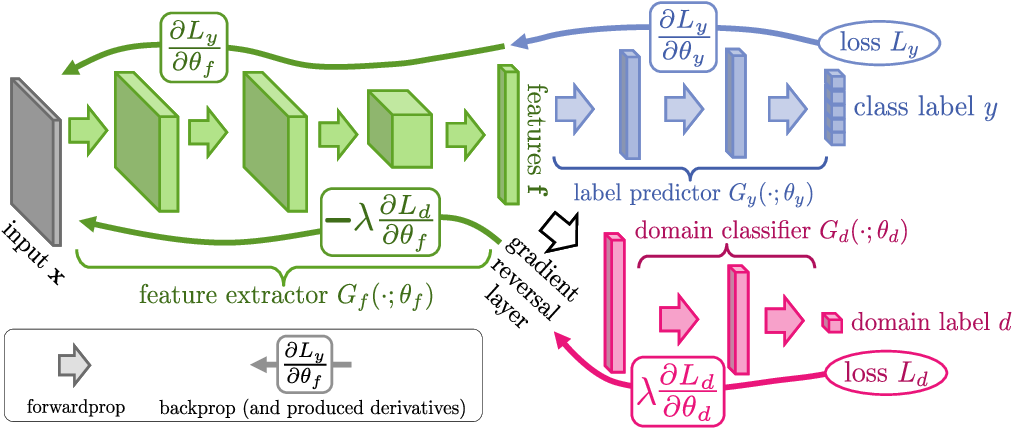
\includegraphics[width=\textwidth]{abbildungen/dann.png}
  \caption{Domain-Adversarial Training \cite{dannGanin}: In the domain-adversarial training of a network, the features are first extracted from the input. Then these extracted features are both used to train the label predictor to be able to make accurate predictions of the class of the input and, at the same time, to try to confuse the domain classifier to make bad predictions about the domain of the input. Both classifiers are trained adversarially against each other.}
  \label{fig:dann}
\end{figure}

As describe above, the DANN has to learn to classify images as accurately as it can while not classifying their domains well. The accuration of the classification can be measured by a loss function that indicates how far the prediction is from the reality. To classify the image, it learns to minimize the classification loss $\mathcal{L}(\bm{f}(\bm{x}), y)$ defined using the negative log probability as in equation \ref{eq:neglogDANN} where $f(\bm{x})$ is the predicted probability of $x$ being in class $y$ defined by the softmax function as in \ref{eq:softmaxDANN} 
 	\begin{equation} \label{eq:neglogDANN}
			\mathcal{L}(\bm{f}(\bm{x}), y) = log\frac{1}{f_y(\bm{x})}
	\end{equation} 	
	\begin{equation} \label{eq:softmaxDANN}
			\bm{f}(\bm{x}) = softmax(\bm{c} + \bm{V}h(x)),
			softmax(\bm{a}) = \left[\frac{1}{1+exp(a_i)}\right]_{i=1}^{|\bm{a}|}
	\end{equation}
	\begin{equation} \label{eq:represDANN}
			\bm{h}(\bm{x}) = sigm(\bm{b} + \bm{W}h(x)), 
			sigm(\bm{a}) = \left[\frac{exp(a_i)}{\overset{|\bm{a}|}{\underset{j=1}{\sum}}exp(\bm{a}_j)}\right]_{i=1}^{|\bm{a}|}
	\end{equation}
$h(\cdot)$ in \ref{eq:represDANN} can be viewed as the internal representation of the neural network responding to the $m$ labeled source data: $\bm{h}(S) = \left\{\bm{h}(\bm{x}_i^s)\right\}_{i=1}^m$. Then, $\bm{b}, \bm{W}$ are the network parameters responsible for creating the representations and $\bm{c}, \bm{V}$ are parameters of the classifier similar to $\bm{b}, \bm{W}$ 

Then we have unlabeled data from the target domain with $n$ samples and the representation $\bm{h}(T) = \left\{ \bm{h}(\bm{x}_i^t)\right\}_{i=1}^{n}$. Combining the empirical $\mathcal{H}$-divergence \cite{DArepres, H-Kifer}, a method to measure the difference of data distribution, measuring the difference between the representations $\bm{h}(S)$ and $\bm{h}(T)$ \eqref{eq:hDiv} and a logistic regressor predicting the probability of a given output being from the source domain or target domain, $z = 1$ or $z = 0$ accordingly \eqref{eq:logReg}:
 	\begin{equation} \label{eq:hDiv} 
			\hat{d}_{\mathcal{H}} = 2\left(1 - \underset{min}{\eta \in \mathcal{H}}\left[\frac{1}{m}\underset{i=1}{\overset{m}{\sum}}I\left[\eta \left(\bm{h}\right(\bm{x}_i^s)) = 1\right] + \frac{1}{n}\underset{i=1}{\overset{n}{\sum}}I\left[\eta \left(\bm{h}\left(\bm{x}_i^t\right)\right) = 0\right]\right]\right) 
	\end{equation} 
	\begin{equation} \label{eq:logReg} 
			p(z =1 | \Phi) = o(\Phi) = sigm(d+\bm{u}^T\Phi), \Phi \in \left\{\bm{h}(\bm{x}_i^s), \bm{h}(\bm{x}_i^t)\right\}
	\end{equation} 
with weights and biases of the neurons $\bm{u}, d responsible for the domain regressor$.

Regarding both parts, the classifier and the domain regressor, the DANN tries to minimize the loss of the first and to maximize the confusion in the second. The optimization problem its training has to solve is as follow:
	\begin{equation} \label{eq:optDANN} 
			\underset{\bm{b}, \bm{c}, \bm{V}, \bm{W}}{min}\frac{1}{m}\underset{i=1}{\overset{m}{\sum}}\mathcal{L}\left(\bm{f}\left(\bm{x}_i^s\right), y_i^s\right) + \lambda\underset{\bm{u}, d}{max}\left[\left(-\frac{1}{m}\underset{i=1}{\overset{m}{\sum}}\mathcal{L}^d\left(o\left(\bm{x}_i^s\right), 1\right) - \frac{1}{n}\underset{i=1}{\overset{n}{\sum}}\mathcal{L}^d\left(o\left(\bm{x}_i^t\right), 0\right)\right)\right]
	\end{equation} 


% Loss Functions
\section{Loss Functions of Domain Separation Networks} \label{sec:dsnLoss}
The loss function gives information about how well the network can already classify the given data. It can be defined to evaluate the error of the network and to lead the learning in the direction we want. The total loss of DSN is defined as follow 
	\begin{equation} \label{eq:lossesDSN}
			\mathcal{L} = \mathcal{L}_{Task} + \alpha \mathcal{L}_{recon} + \beta \mathcal{L}_{difference} + \gamma \mathcal{L}_{similarity}
	\end{equation}
where $\alpha$, $\beta$ and $\gamma$ are coefficients for the reconstruction loss $\mathcal{L}_{recon}$, the difference loss $\mathcal{L}_{difference}$ and the similarity loss $\mathcal{L}_{similarity}$ respectively. 

Now that we know all the necessary components and the overall loss function, the definitions of all the loss functions will be declared and explained.

\subsection*{Task loss}
For the main task of image classification, we want the network to make accurate predictions regarding the class of an image. If there is a dog in a picture, the network should predict that it is highly probable that a dog is in that picture. If the prediction indicates otherwise, there must be a noticeable consequence. Having the ground-truth information, the labeled data, one way to do this is to define a loss function indicating the amount of errors in the predictions: the further the predictions are from the reality, the bigger the loss is. The authors use the negative log-likelihood as defined in equation \eqref{eq:loglikeFnc} for the task loss $\mathcal{L}_{Task}$.
	\begin{equation} \label{eq:loglikeFnc}
			\mathcal{L}_{Task} = -\overset{N_s}{\underset{i = 0}{\sum}}y_i^s \cdot log {\hat{y}_i}^s
	\end{equation}

where  $y_i^s$ is the class label in one-hot encoding form for input $i$ and ${\hat{y}_i}^s$ the softmax prediction of the classifier $G\left(E_c(x^s)\right)$.

The negative log-likelihood is bigger, when the predicted probability of an image belonging to a wrong class is high or when the predicted probability of the right class is low. Therefore, the network learns to adjust its parameters to minimize this loss - to make more accurate predictions. It must be note that this classification loss is calculated based only on the labeled source data offering ground-truth information.

\subsection*{Difference Loss}
The difference loss encourages the private encoders and the shared encoders to be different. They should capture other aspects of the same input from both domains. Here, the authors use a soft subspace orthogonality constraint between the two representations of each domain. The difference loss is defined as:
	\begin{equation} \label{eq:difflossFnc}
			\mathcal{L}_{difference} = \Vert {H_c^s}^T{H_p^s}{\Vert_F^2} + \Vert {H_c^t}^T{H_p^t}{\Vert_F^2}
	\end{equation}
	\begin{equation} \label{eq:frebFnc}
			\Vert A {\Vert_F} = \sqrt{\overset{m}{\underset{i = 1}{\sum}}\overset{n}{\underset{j = 1}{\sum}}|a_{ij}|^2}
	\end{equation}

where ${H_c^s}$ and ${H_p^s}$ are matrices which respectively has the hidden shared representations $h_c^s = E_c(x^s)$ and the private representation $h_p^s = E_p(x^s)$ of the samples from the source domain as their rows and ${H_c^t}$ and ${H_p^t}$ are matrices with the hidden shared representations $h_c^t = E_c(x^t)$ and the private representation $h_p^t = E_p(x^t)$ of those from the target domain as their rows respectively. $\Vert \cdot {\Vert_F^2}$ is the squared Frobenius Norm with \eqref{eq:frebFnc} as definition.

\subsection*{Reconstruction Loss}
DSN has a structure generating domain-specific representations which are held apart from the shared representation by the difference losses. To ensure that the private representations are not trivial, the authors also add reconstruction loss using scale-invariant mean squared error $\mathcal{L}_{si}$\_${mse}$ as defined in equation \eqref{eq:reclossFnc} and \eqref{eq:si_mse}
	\begin{equation} \label{eq:reclossFnc}
			\mathcal{L}_{recon} = \overset{N_s}{\underset{i = 1}{\sum}}{\mathcal{L}}_{si\_{mse}}(x_i^s, {\hat{x}_i}^s) + \overset{N_t}{\underset{i = 1}{\sum}}{\mathcal{L}}_{si\_{mse}}(x_i^t, {\hat{x}_i}^t)
	\end{equation}		

	\begin{equation} \label{eq:si_mse}
			\mathcal{L}_{si\_{mse}}(x_i^s, {\hat{x}_i}^s) = \frac{1}{k} \Vert x - \hat{x}{\Vert_2^2} - \frac{1}{k^2} ([x - \hat{x}] \cdot 1_k)^2
	\end{equation}

	\begin{equation} \label{eq:L2Fnc}
			x = \left(\begin{array}{c} x_1\\ x_2\\ \vdots \\ x_n \end{array} \right),
			\Vert x {\Vert_2^2} = \sqrt{\overset{n}{\underset{k = 1}{\sum}}{|x_k|}^2} \\
			\mathcal{L}_{si\_{mse}}({x_i}^s, {\hat{x}_i}^s) = \frac{1}{k} \Vert x - \hat{x}{\Vert_2^2} - \frac{1}{k^2} ([x - \hat{x}] \cdot 1_k)^2
	\end{equation}

where $k$ is the pixel number in input $x$, $1_k$ a k-dimensional vector filled with ones, and $\Vert \cdot {\Vert_2}^2$ is the squared $L_2$-norm defined as in equation \ref{eq:L2Fnc}

The authors also proved that by using the scale-invariant mean squared error, better performance can be aimed [DSN]. This is because the scale-invariant mean-squared error allow the DSN to concentrate on reconstructing the shape of the object without being punished on wrong value of intensity or absolute color whereas the traditional mean-squared error also punishes wrong scaling of the output despite the object being reproduced correctly. 

Pictures can also be regenerated back according to the diffrerent representations as shown in Figure \ref{fig:reconImg}

\begin{figure}[tbh]
  \centering
    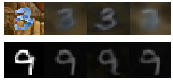
\includegraphics[width=0.6\textwidth]{abbildungen/reconPic.png}
  \caption{Reconstructed Images: These are the images reconstructed from different representations. Respectively from the left to the right of each row, the first one is the original image, the second is reconstructed from both the shared and private representations, the third is from only the shared representations and finally, the fourth is constructed only after the private representations.}
\label{fig:reconImg}
\end{figure}

\subsection*{Similarity Loss}
For the shared representations, both the representations of the samples from the source domain and of the samples from the target domain should be similar. In that way, the classifier can train on the common representations that are domain-independent. To induce this in the model, the authors chose two ways to define the similarity loss: the domain adversarial similarity loss and the maximum mean discrepancy. 

\paragraph*{i. Domain Adversarial Similarity Loss} This adversarial learning is also known in Domain Adversarial Neural Network (DANN) \cite{DAGanin} described previously in \ref{sec:dann}. It is a way to induce the similar representations of both domains is by learning to create representations that confuse a domain classifier. On one side, there is a domain classifier learning to predict the domain of the samples from the encoded representations. On the other side, the representations should be created so that the classifier cannot reliably predict their origin domain. 

To enable this contrary behavior in the model, the Gradient Reversal Layer (GRL) is used. The GRL $Q(f(u))$ is defined as the identity function $f(x) = x$ but has the reversed gradient direction, that is: 
	\begin{equation}
			Q(f(u)) = f(u)
	\end{equation}

	\begin{equation}
			\frac{d}{du}Q(f(u)) = -\frac{d}{du}Q(f(u)) = -\frac{d}{du}f(u)
	\end{equation}

Formally, there is the domain classifier $Z(Q(h_c);\bm{\theta}_z) \rightarrow \hat{d}$ making prediction on the domain $\hat{d} \in \left\{0, 1\right\}$ of the input sample x through a shared representation vector $h_c = E_c(x; \bm{\theta}_c)$. While $\bm{\theta}_z$ is adjusted to improve accuracy of the classifier in predicting the domain of the encoded images, the parameters $\bm{\theta}_c$ are optimized to create representations that the classifier cannot classify accurately. 

\paragraph*{ii. Maximum Mean Discrepancy} 
Maximum Mean Discrepancy (MMD) is a kernel-based method proposed by \cite{mmdOrig} to find out if the two drawn samples are from the same distribution. This problem is also known as the two-sample problem and is defined formally as: given $X := \left\{x_1, \cdots, x_m\right\}$ drawn from $p$ and $Z := \left\{z_1, \cdots, z_m\right\}$ drawn from $q$, we want to test whether $p=q$ \cite{mmdbio}. 

Generally, MMD is the maximum difference of the mean function value $f(x)$ and $f(y)$ on samples $X$ and $Y$. Since we want to concentrate on the usage of the MMD, the derivation of the equation \eqref{eq:mmddsnFnc} used in the DSN will not be explained in detail here but can be found in \cite{mmdOrig}. Here, the authors used the biased statistic for the squared population MMD to measure the difference between the shared representations of the samples from the source domain $\bm{h}_c^s$ and the shared representations of those from the target domain $\bm{h}_c^t$:
\begin{equation}\label{eq:mmddsnFnc}
			\mathcal{L}_{similarity}^{MMD} = \frac{1}{(N^s)^2}\overset{N^s}{\underset{i, j = 0}{\sum}}k(\bm{h}_{ci}^s, \bm{h}_{cj}^s) - \frac{2}{N^sN^t}\overset{N^s, N^t}{\underset{i, j = 0}{\sum}}k(\bm{h}_{ci}^s, \bm{h}_{cj}^t) + \frac{1}{(N^t)^2}\overset{N^t}{\underset{i, j = 0}{\sum}}k(\bm{h}_{ci}^t, \bm{h}_{cj}^t)
	\end{equation} 
with a positive definite kernel function $k(\cdot, \cdot)$. The author chose a linear combination of multiple radial basis function kernel defined as: 
\begin{equation}\label{eq:rbfFnc}
			k(x_i, x_j) = \sum_n \eta_n exp\left\{-\frac{1}{2\sigma_n}\Vert x_i - x_j\Vert^2\right\} 
	\end{equation} 
with the standard deviation $\sigma_n$ and the weight of the $n^{th}$ kernel $\eta_n$  

After the introduction to the components of the DSN, we can summarize it as follow: the encoders, the decoders and the classifier along with the difference loss, the reconstruction loss, and the similarity loss  enable the DSN to be trained to apply domain adaption to image classification. The private encoders for the source and target domains $E_p^s(\bm{x}^s)$ and $E_p^s(\bm{x}^s)$ create the private source representations $\bm{h}_p^s$ to be different to the shared representations also built from the source $\bm{h}_c^s$, and the private target representations $\bm{h}_p^t$ to also be different to the shared representations from the target domain $\bm{h}_c^t$. The differences between these representations are induced by the difference loss $\mathcal{L}_{difference}$. At the same time, the similarity loss $\mathcal{L}_{similarity}$supports the similarity between both shared representations $\bm{h}_c^s$ and $\bm{h}_c^t$ on which the classifier can train effectively according to a theory to domain adaptation described in Section \ref{ch:domainAdaptation}. Then, to prevent the private encoders from creating trivial solutions trying to be different from the shared representations, the reconstruction loss is added to ensure that the encoded matrices can still be decoded back to images resembling the ones from their domain of origin. Finally, the classifier trains to classify image by learning from the domain-invariant representations created by the share encoders as mentioned before. Their cooperation is depicted in figure \ref{fig:DSN}.

\section{Previous Experiments with Domain Separation Networks} 
\subsection*{Domain Separation Networks (DSN)} In the original paper, the authors are interested in the DSN's performance on a real-world dataset when it is trained on a synthetic data. This scenario involves domain transfer from a domain with clear representation of data to the noisy one. The dataset they used are MNIST, white digits on black backgrounds, MNIST-M created by inverting color of the images in MNIST partially. They carry experiments using DSN trained on MNIST \cite{mnist} to test on MNIST-M \cite{mnist-m}, Synthetic Digits to the Street View House-Number Set (SVHN) \cite{svhn}, SVHN to MNIST, Synthetic Signs to the real-world dataset of traffic signs (GTSRB) \cite{gtsrb} and synthetic objects to LINEMOD \cite{linemod}. Samles from some of these datasets can be seen in figure \ref{fig:datasets}. 

As they reported, they achieved the highest classification accuracy when using the DSN with the DANN as similarity loss. This shows the effectiveness of their domain adaptation method separating domain-specific information from the shared representation.

\begin{figure}[tbh]
  \centering
    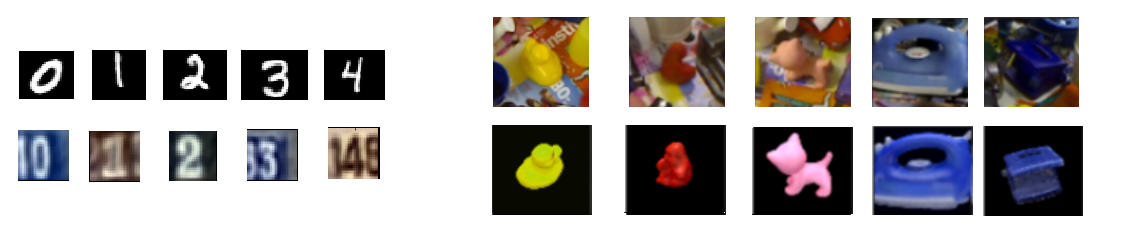
\includegraphics[width=\textwidth]{abbildungen/datasets.png}
  \caption{Synthetic Images and Real-world Images: On the left, samples from the MNIST dataset (upper left) and from the SVHN (lower left) are shown. We can see that the first has cleaner look with clear digits and uniform background while the real-world house numbers have blurry appearance. Similarly on the right, the synthetic objects (upper right) has black background and the objects from the LineMod (lower right) are almost lost among the background, as pictures from the real scene could look like.}
  \label{fig:datasets}
\end{figure}

\subsection*{Speech Recognition with DSN \cite{dsnspeech}} 
The DSN has found not only application in computer vision, but also in speech recognition. In this paper, it is used in an unsupervised domain adaptation problem to recognize speeches with only a sequence of speech with labels. They also train the network on a clean speech data and test on the noisy speech data. Also this work reports a good average performance of the DSN in the speech recognition. Since this is not exactly our scope, we will not go in the detail of this work. Further information can be found in \cite{dsnspeech}. 

After knowing the components and functions of the DSN in this section, how it extracts features specific to each domain and hold it far from each other and at the same time extract shared aspects of both domains, it is imaginable that the domain separation network would be a suitable choice for this situation.  the DSN has encoders which learn to explicitly extract the domain-specific information on both domains. This way, it can really tell both domains apart even if they are mixed together. Besides, by extracting the private representations of each domain, it can make clearer representations of the objects even though it has not seen labeled image of that object from another domain before. The DSN extracts the characters of each domain and create the representations freed from the domains on which its classifier can learn about the objects very precisely without noises from both the differences an the similarities between the domains. In the next section, we will introduce our experiments using this network and present our results.

In our experiment, the complete domain mixture scenario, with both domains having samples from all classes, is investigated. The main difference to \cite{domainMixture} is that another neural network architecture is used to observe the effect of this mixture. While they train a DANN on these scenarios in \cite{domainMixture}, the DSN is used in this thesis. Practically, the DSN also includes the DANN to create domain-free representations, then additionally create domain-specific representations. By using another neural network, we can also see if the interference of the mixture they measure is specific to the choice of the model or not and how. The experiments will also be carried with different number of classes from which each domain has supervised samples to see how the overlapping of the data of the same object between the domains influences the performance of the model. The next section will describe our experimental setup further in details.